\chapter{Resultados} \label{ch:RD}

A estatística descritiva do atributo SST é mostrada na Tabela \ref{tbl:sst_stat}, onde nota-se uma grande variabilidade nos dados. Dessa forma, é possível construir um modelo robusto capaz de realizar a predição deste atributo para diferentes estádios de maturação da manga.

\begin{table}[H]
\centering
\caption{Estatística descritivas dos valores de referência de SST.} \label{tbl:sst_stat}
\begin{tabular}{llllllll}
\hline
Dados     & Amostras & M\'edia & M\'in & M\'ax & Amplitude & SD & Vari\^ancia   \\
\hline
SST     & 1200 & 9,83 &  3,8 &  19,7 &  15,9 &  4,5 &  20,24 \\
\hline
\end{tabular}
\legend{\textbf{Fonte: } (Autor, 2019).}
\end{table}

Inicialmente os modelos construídos na literatura foram replicados para as mangas Palmer, para a comparação dos resultados. No trabalho de Khairunniza-Bejo e Kamarudin (2011), o atributo SST foi previsto em mangas Chokanan a partir do espaço de cores HSV. Os autores construíram modelos de Regressão Linear Simples para cada canal deste espaço de cor, e obtiveram como melhor resultado um coeficiente de correlação igual a -0,92 para o canal matiz. Assim, para as mangas da variedade Palmer, também foi construída uma Regressão linear com o atributo matiz como entrada. Entretanto, esperava-se um resultado inferior aos obtidos pelos autores, visto que, para as mangas Palmer, o atributo matiz não varia linearmente. A Figura \ref{fig:hue_sst} mostra a variação do SST de acordo com a matiz. 

\begin{figure}[H]
\centering
	\caption{Variação do SST conforme a matiz.}
	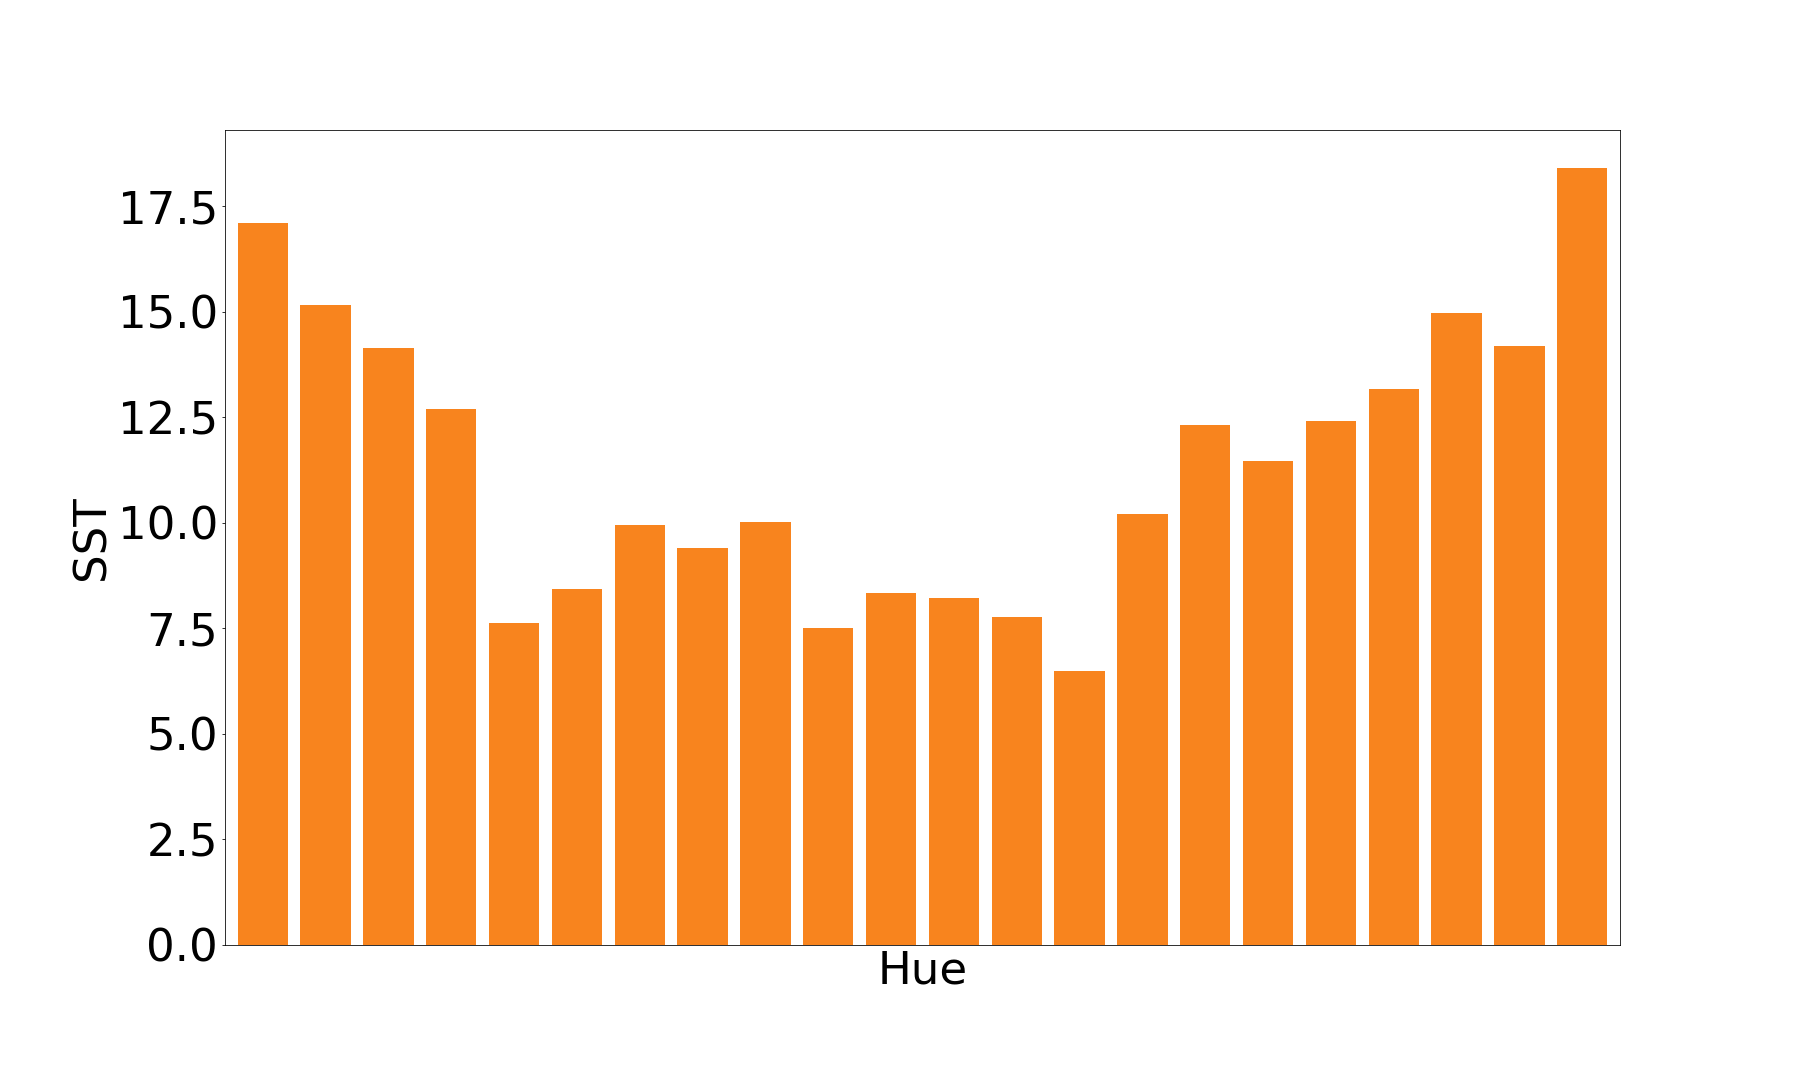
\includegraphics[scale=0.18]{img/hue_sst_palmer.png}
	\legend{\textbf{Fonte:} (Autor, 2019).}\label{fig:hue_sst}
\end{figure}

Conforme esperado, o coeficiente de correlação obtido para a Regressão linear foi muito inferior, com um valor igual a -0,1179. Na Figura \ref{fig:comp_hue}, são mostradas a reta ajustada para as amostras do presente estudo e a reta ajustada pelos autores Khairunniza-Bejo e Kamarudin (2011). 

\begin{figure}[H]
\centering
    \caption{\label{fig:comp_hue} Modelos de Regressão linear construídos para o atributo matiz (a) Presente estudo (b) Trabalho de Khairunniza-Bejo e Kamarudin (2011).}
    \subcaptionbox{}{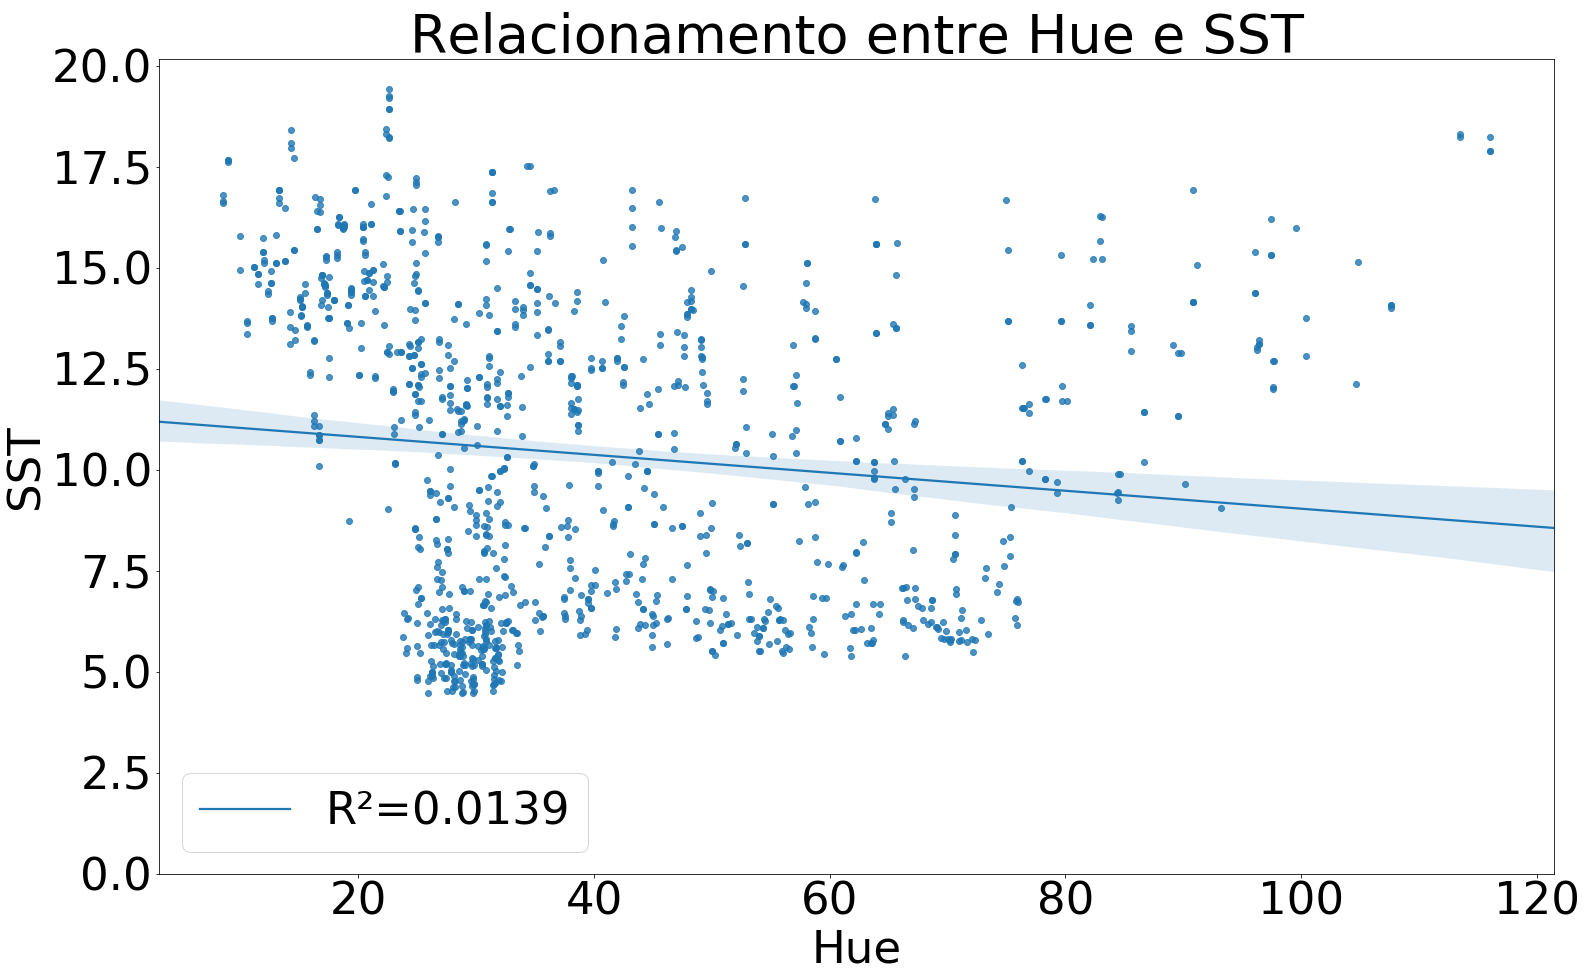
\includegraphics[scale=0.133]{img/scatter_sst_hue_palmer.png}}
    \subcaptionbox{}{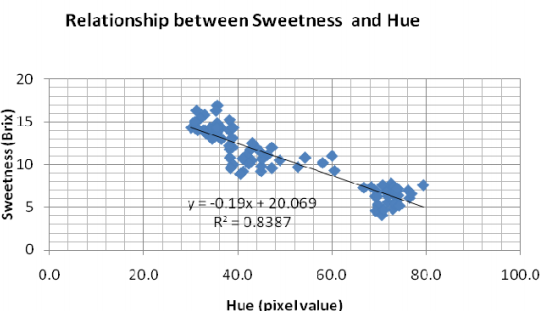
\includegraphics[scale=0.4]{img/sst_lit_hue.png}}
    \legend{\textbf{Fonte: } (Autor, 2019; Khairunniza-Bejo, Kamarudin, 2011).}
\end{figure}

Devido ao relacionamento não linear entre a matiz e SST, esperava-se que com a \textit{Random Forest} fosse obtido um resultado superior. Os valores de $R$ e $RMSE$ obtidos por ela e pela Regressão linear, para cada \textit{fold}, são mostrados na Figura \ref{fig:fold_sst_hue}.

\begin{figure}[H]
\centering
	\caption{Resultados obtidos para a matiz (a) Coeficiente de correlação (R) (b) RMSE.}
	\subcaptionbox{}{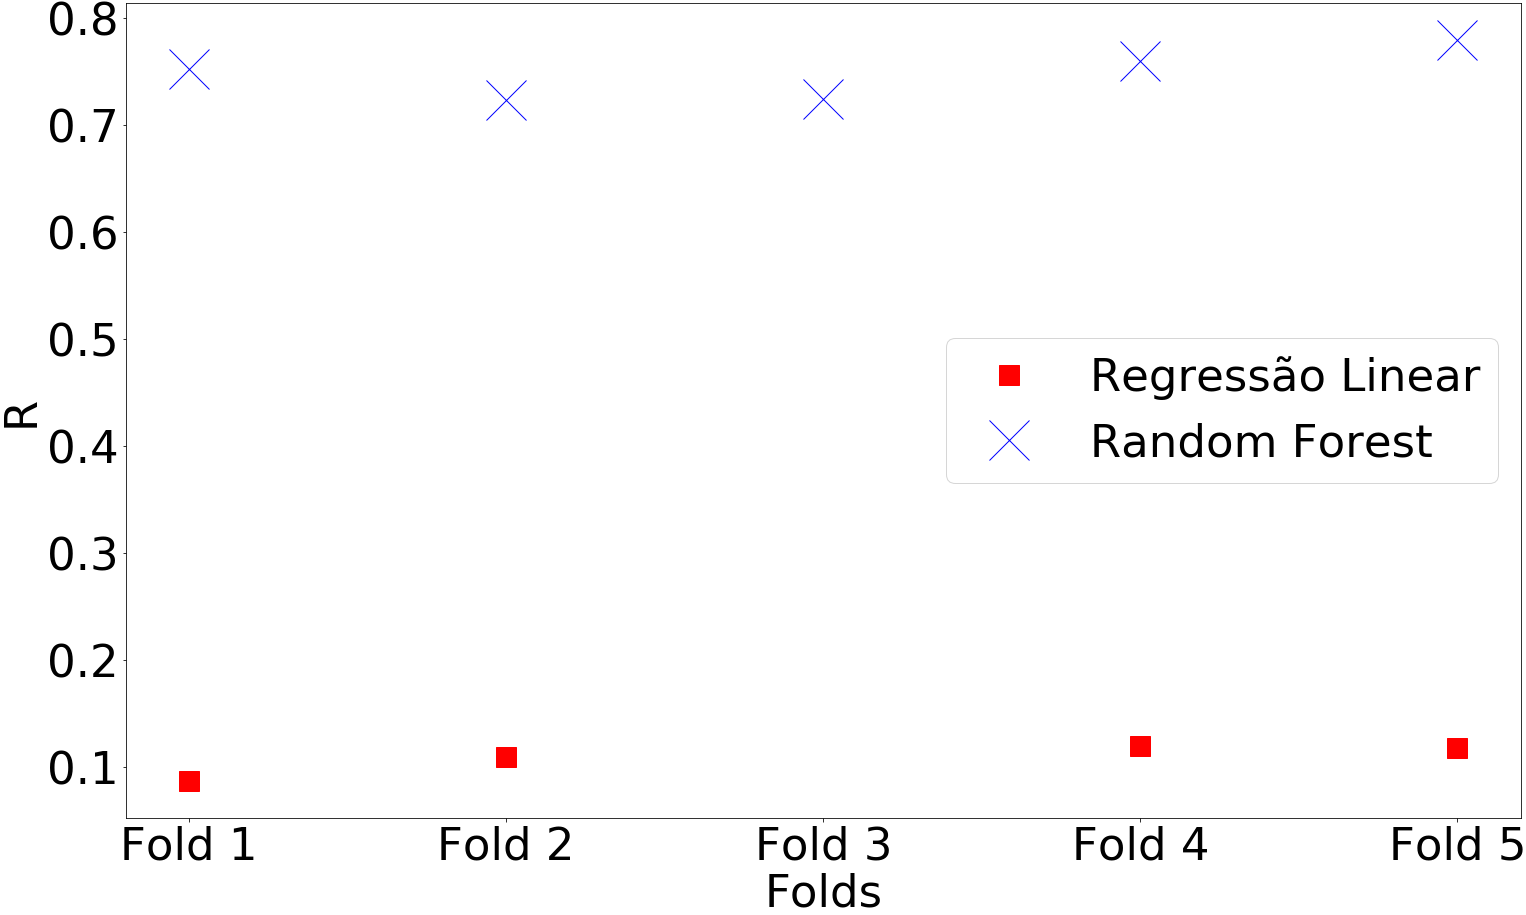
\includegraphics[scale=0.14]{img/fold_r_sst_hue_palmer.png}}
	\subcaptionbox{}{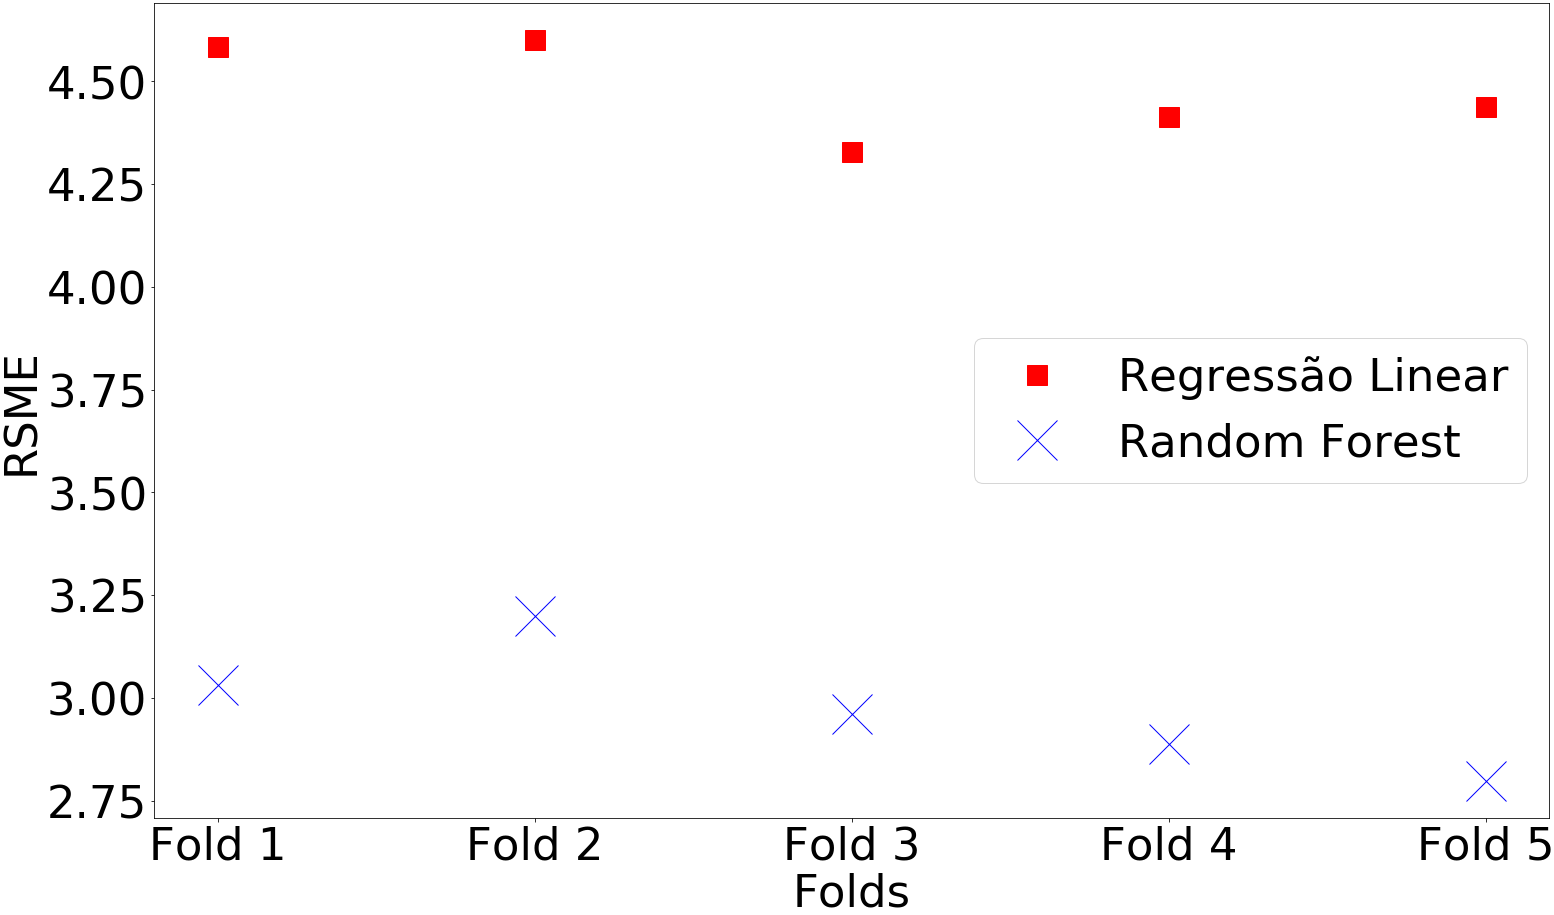
\includegraphics[scale=0.14]{img/fold_rmse_sst_hue_palmer.png}}
	\legend{\textbf{Fonte:} (Autor, 2019).}\label{fig:fold_sst_hue}
\end{figure}

Apesar de a \textit{Random Forest} ser claramente superior à MLR, como esperado, o resultado ainda é inferior ao obtido pelos autores. Enquanto eles alcançaram um coeficiente de correlação igual a -0,92, o coeficiente médio obtido pela técnica \textit{ensemble} não alcançou o valor de 0,8. Ademais, o RMSE obtido no estudo é muito maior que o obtido por eles (0,033 ºBrix). Para as mangas da variedade Palmer, vê-se que este atributo não é suficiente para a determinação de SST como foi para as mangas da variedade Chokanan.

Por outro lado, os autores Yahaya et al. (2015) testaram o espaço de cores RGB e obtiveram um coeficiente de correlação igual a 0,814 e RMSE igual a 1,218 ªBrix em mangas da variedade Sala. Para verificar se existe uma relação linear entre as variáveis RGB extraídas das mangas Palmer e o SST, foram plotadas as variações das mesmas, mostradas na Figura \ref{fig:rgb_sst}.

\begin{figure}[H]
\centering
    \caption{\label{fig:rgb_sst} Variação do SST conforme as variáveis RGB (a) Canal R (b) Canal G (c) Canal B.}
    \subcaptionbox{}{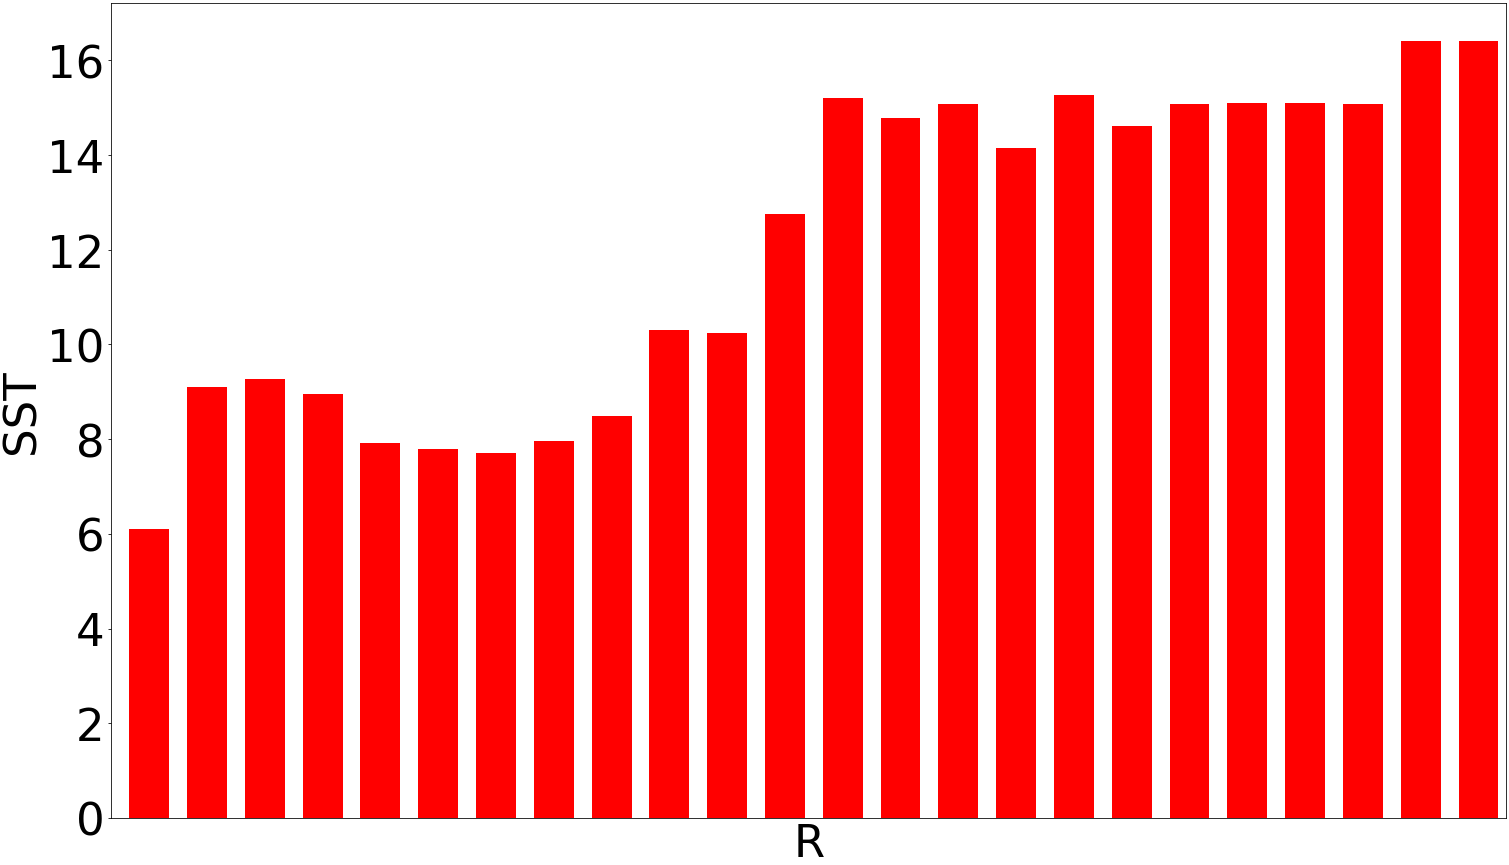
\includegraphics[scale=0.12]{img/R_sst_palmer.png}}
    \subcaptionbox{}{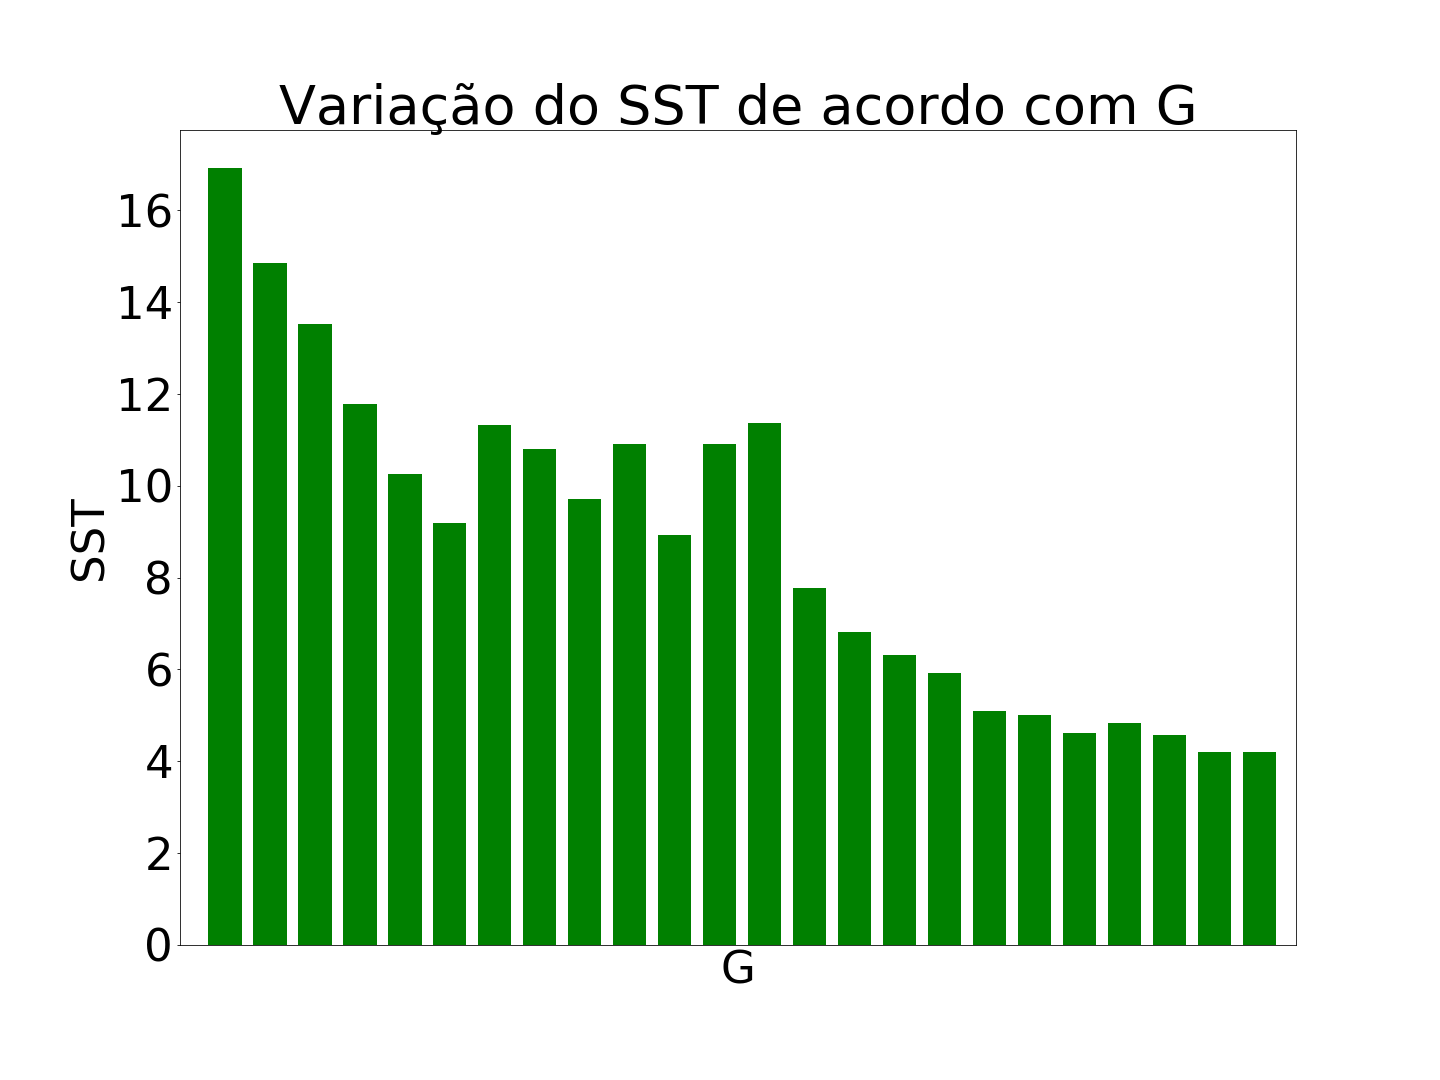
\includegraphics[scale=0.12]{img/G_sst_palmer.png}}
    \subcaptionbox{}{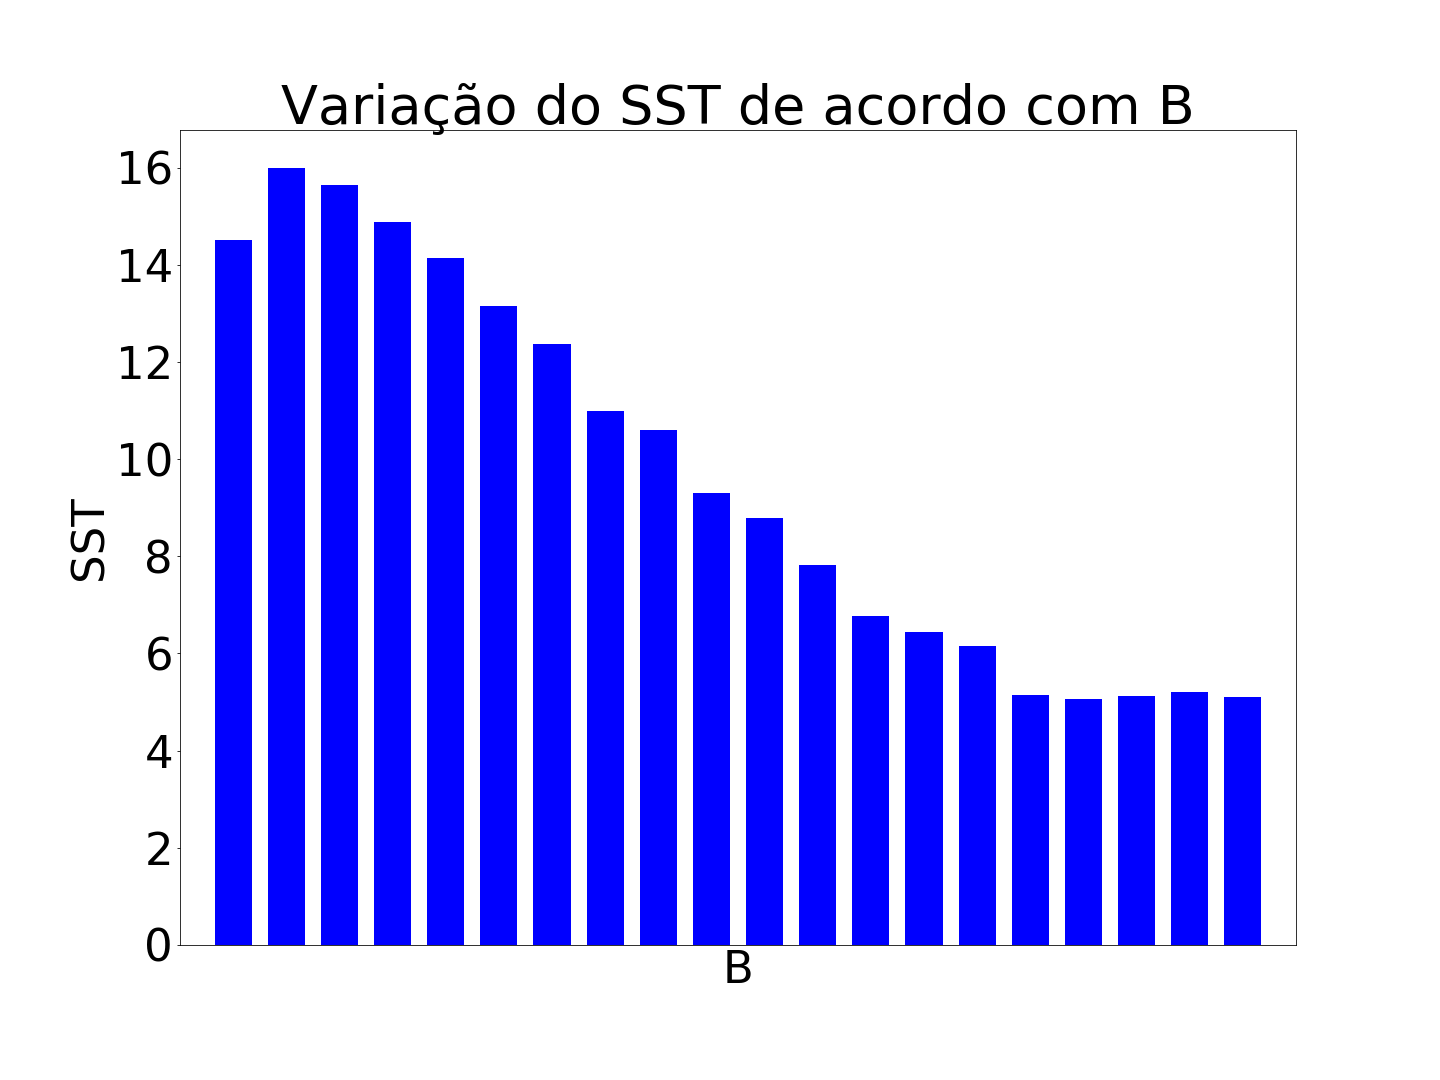
\includegraphics[scale=0.12]{img/B_sst_palmer.png}}
    \legend{\textbf{Fonte: } (Autor, 2019).}
\end{figure}

Nota-se um comportamento aproximadamente linear para as três variáveis. Assim, esperava-se que, através da Regressão Linear Múltipla, fosse obtido um coeficiente de correlação maior que o obtido para a matiz.  Na Figura \ref{fig:fold_sst_rgb}, são mostrados os valores de R e RMSE para a Regressão Linear e também a \textit{Random Forest} em todos os \textit{folds}.

\begin{figure}[H]
\centering
	\caption{Resultados obtidos para as variáveis RGB (a) Coeficiente de correlação (R) (b) RMSE.}
	\subcaptionbox{}{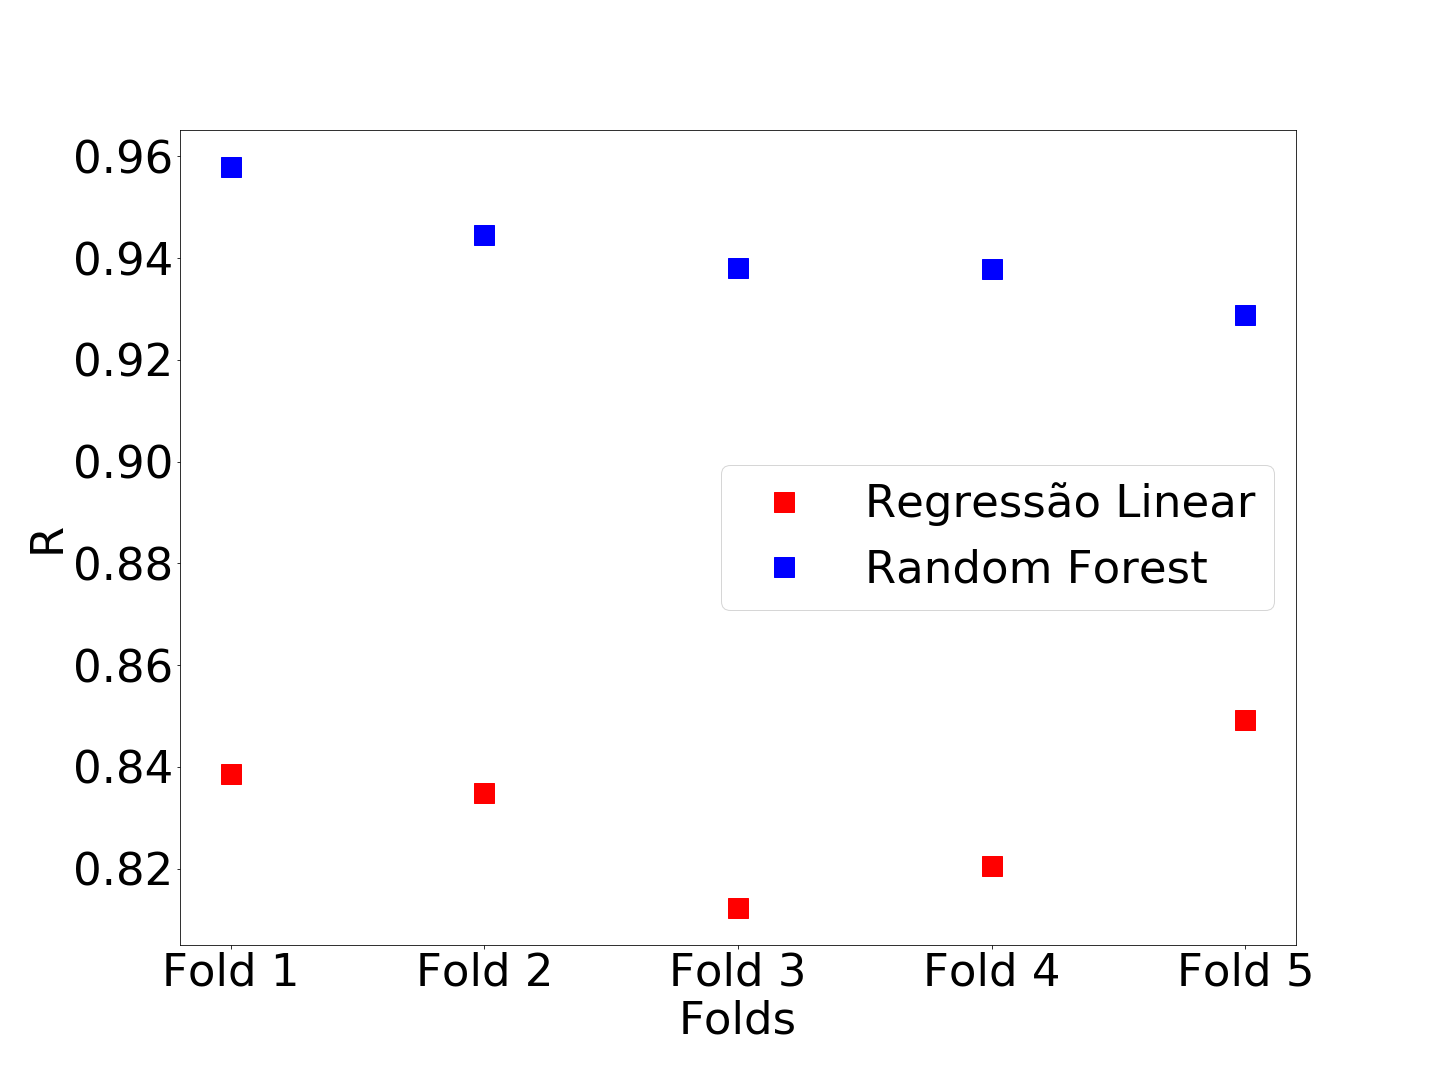
\includegraphics[scale=0.14]{img/fold_r_sst_rgb_palmer.png}}
	\subcaptionbox{}{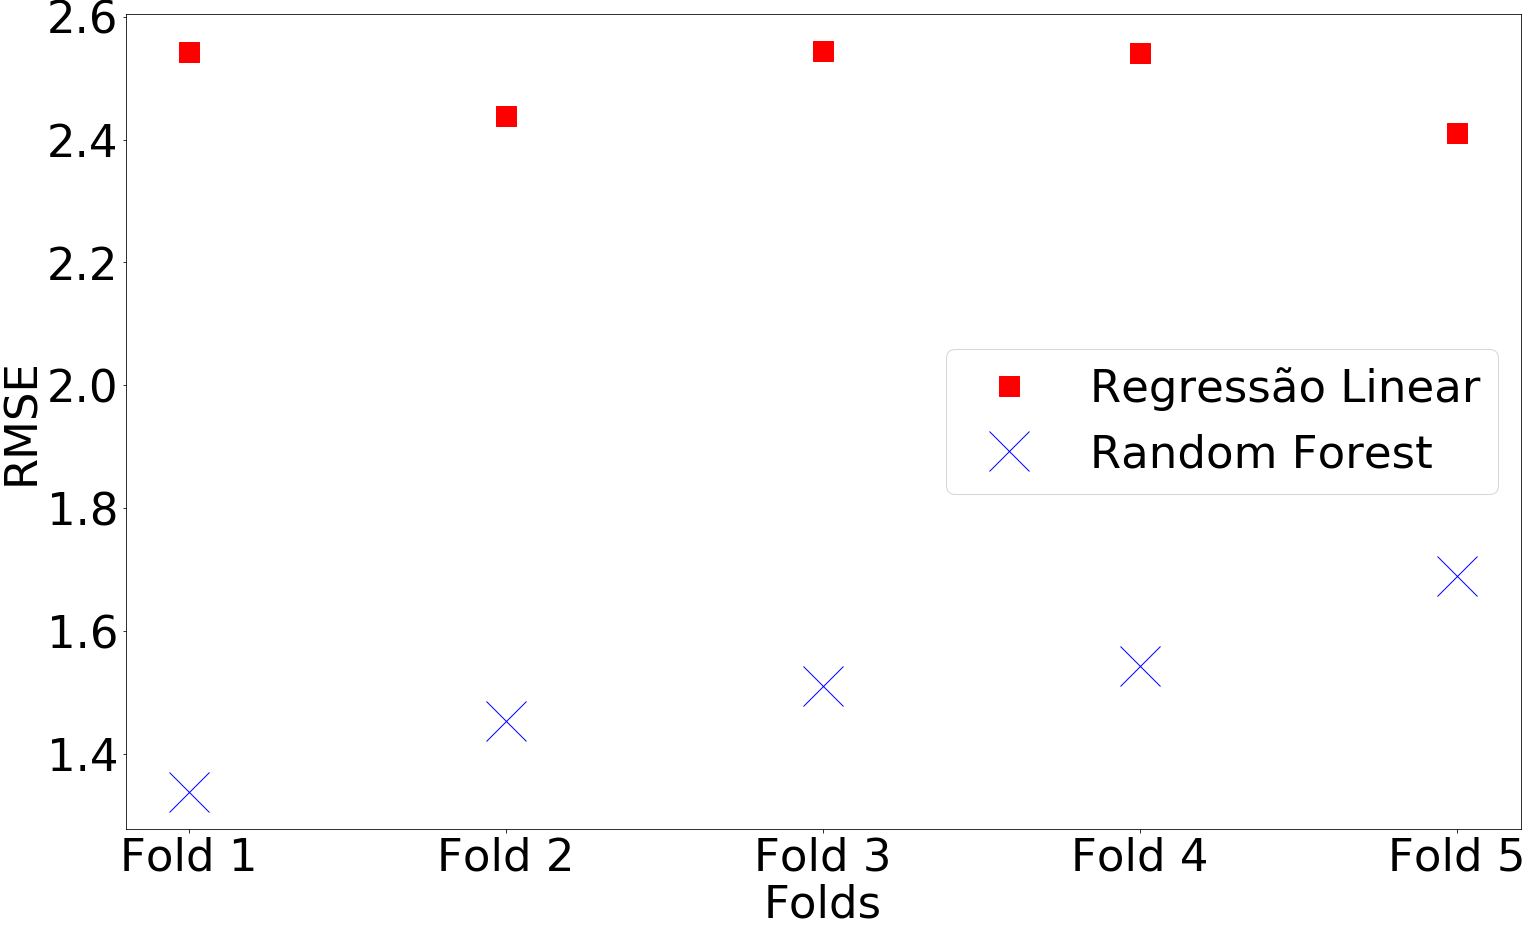
\includegraphics[scale=0.14]{img/fold_rmse_sst_rgb_palmer.png}}
	\legend{\textbf{Fonte:} (Autor, 2019).}\label{fig:fold_sst_rgb}
\end{figure}

Os valores médios dos coeficientes de correlação para a MLR e RF foram, respectivamente, iguais a 0,8312 e 0,9415. Ambas métricas mostraram-se superiores à obtida por Yahaya et al. (2015). Entretanto, o valor de RMSE obtido por eles ainda mostra-se menor que os alcançados para as mangas Palmer.

\section{Modelo com todas as variáveis}

Assim, para a obtenção de um modelo que melhor explique a variação de SST, foi construída uma \textit{Random Forest} com todas as variáveis listadas na Tabela \ref{tbl:var_gps}. Com um maior número de variáveis de entrada, há uma maior quantidade de informações associada à cada manga, aumentando-se assim a probabilidade de alcançar melhores resultados. Da mesma forma, foi construída uma Regressão Linear Múltipla com as mesmas variáveis, de forma a verificar se o relacionamento existente entre as variáveis de entrada e o SST é linear. Os valores de R e RMSE para cada \textit{fold} dos modelos RF e MLR são mostrados na Tabela \ref{tbl:r_rmse_all}.

\begin{table}[H]
	\centering
	\caption{\label{tbl:r_rmse_all} Valores de R e RMSE obtidos pela \textit{Random Forest} e MLR com todas as variáveis.}
	\begin{tabular}{ccccc}
	\hline
	\multirow{2}{*}{\textit{Fold}} & \multicolumn{2}{c}{R} & \multicolumn{2}{c}{RMSE} \\ \cline{2-5}
	  	  & RF      & MLR    & RF 	  & MLR \\ \hline
	1     & 0,9723  & 0.9263 & 1,0018 & 1.61544 \\ \hline
	2     & 0,9405  & 0.9227 & 1,0987 & 1.73668 \\ \hline
	3     & 0,9755  & 0.9219 & 0,7075 & 1.75353 \\ \hline
	4     & 0,9634  & 0.9219 & 0,9029 & 1.82808 \\ \hline
	5     & 0,9660  & 0.9064 & 0,8104 & 1.85705 \\ \hline
	Média & 0,9789 	& 0.9199 & 0,9042 & 1.75816 \\ \hline
	\end{tabular}
	\legend{\textbf{Fonte: } (Autor, 2019).}
\end{table}

Nota-se mais uma vez que o modelo \textit{Random Forest} foi superior à Regressão Linear. O coeficiente de correlação obtido por ele foi maior que o encontrado pelos autores Khairunniza-Bejo e Kamarudin (2011) e Yahaya et al. (2015). Por outro lado, enquanto que o RMSE foi menor que o obtido por Yahaya et al. (2015), ainda foi maior que o RMSE encontrado por Khairunniza-Bejo e Kamarudin (2011) em seu trabalho.

Os atributos mais importantes para a determinação de SST em mangas Palmer podem ser obtidos a partir da propriedade \textit{feature\_importances\_} do \textit{Scikit-Learn}, que retorna um valor de 0 a 1 para cada variável de entrada no modelo RF. Quanto mais próximo de 1 for o valor, mais importante a respectiva variável foi para a construção das regras de decisão da \textit{Random Forest}. Na Figura \ref{fig:feat_import}, são mostradas as variáveis mais importantes do modelo.

\begin{figure}[H]
\centering
	\caption{Atributos mais importantes para a determinação de SST.}
	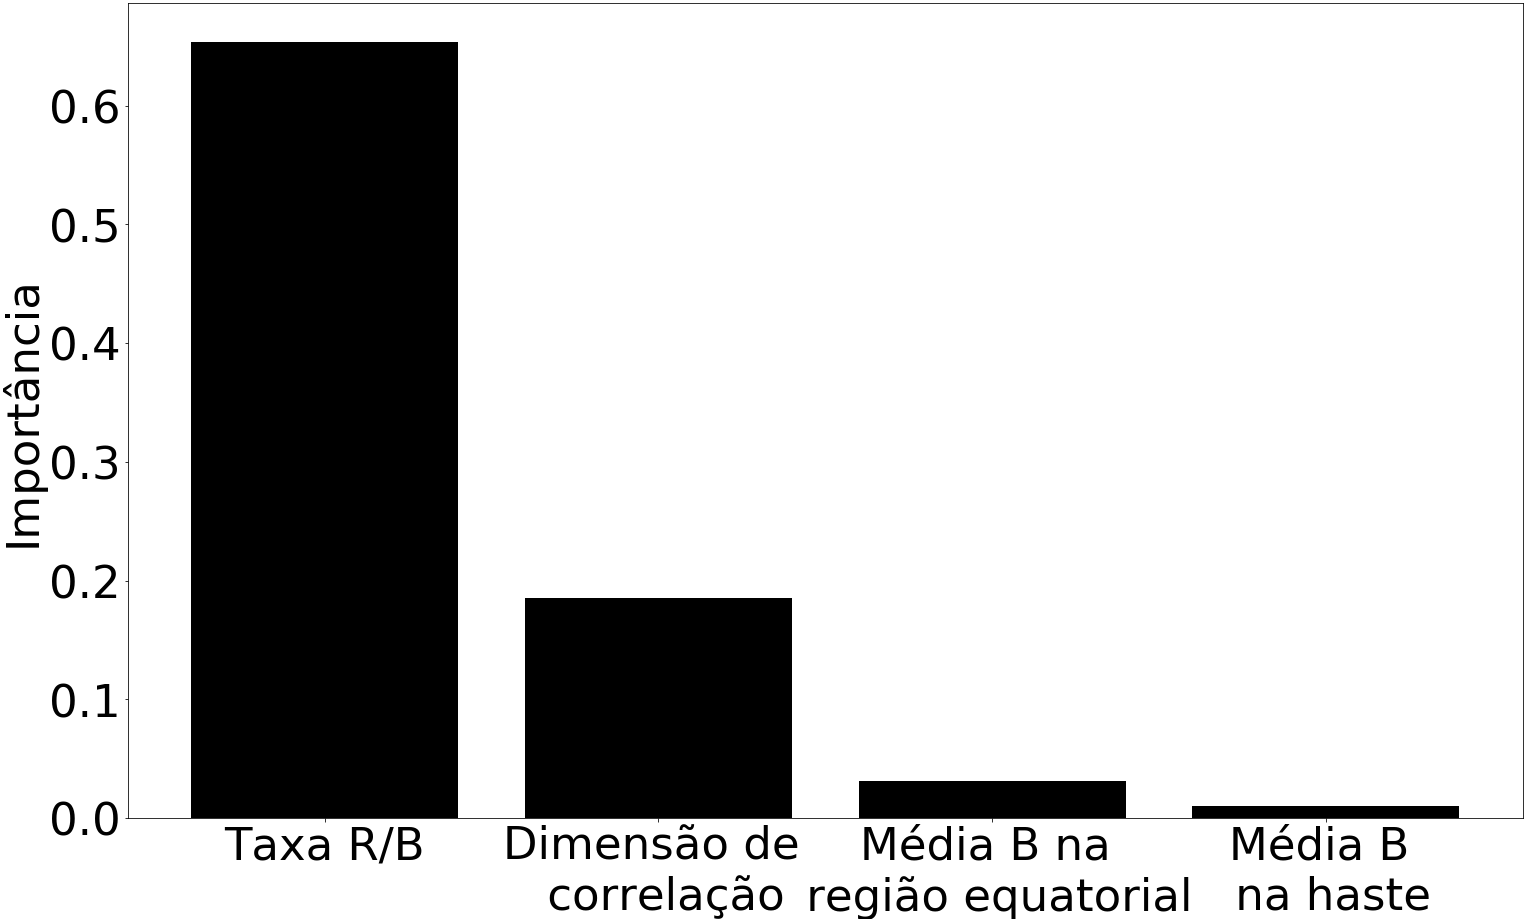
\includegraphics[scale=0.18]{img/feat_import_sst_palmer.png}
	\legend{\textbf{Fonte:} (Autor, 2019).}\label{fig:feat_import}
\end{figure}

Nota-se que o espaço de cores RGB, especialmente o canal B, foi o que mais possuiu relação com o SST. O atributo taxa R/B, que indica a razão entre o valor médio das intensidades no canal R e canal B, mostrou-se o mais significativo. A Figura \ref{fig:rbrate_fig} exibe uma foto em que as intensidades dos pixels originais foram convertidas para R/B. Nota-se, através dela, que a cor arroxeada/amarelada está fortemente associada aos sólidos solúveis totais.

\begin{figure}[H]
\centering
	\caption{Representação de uma foto no canal R/B.}
	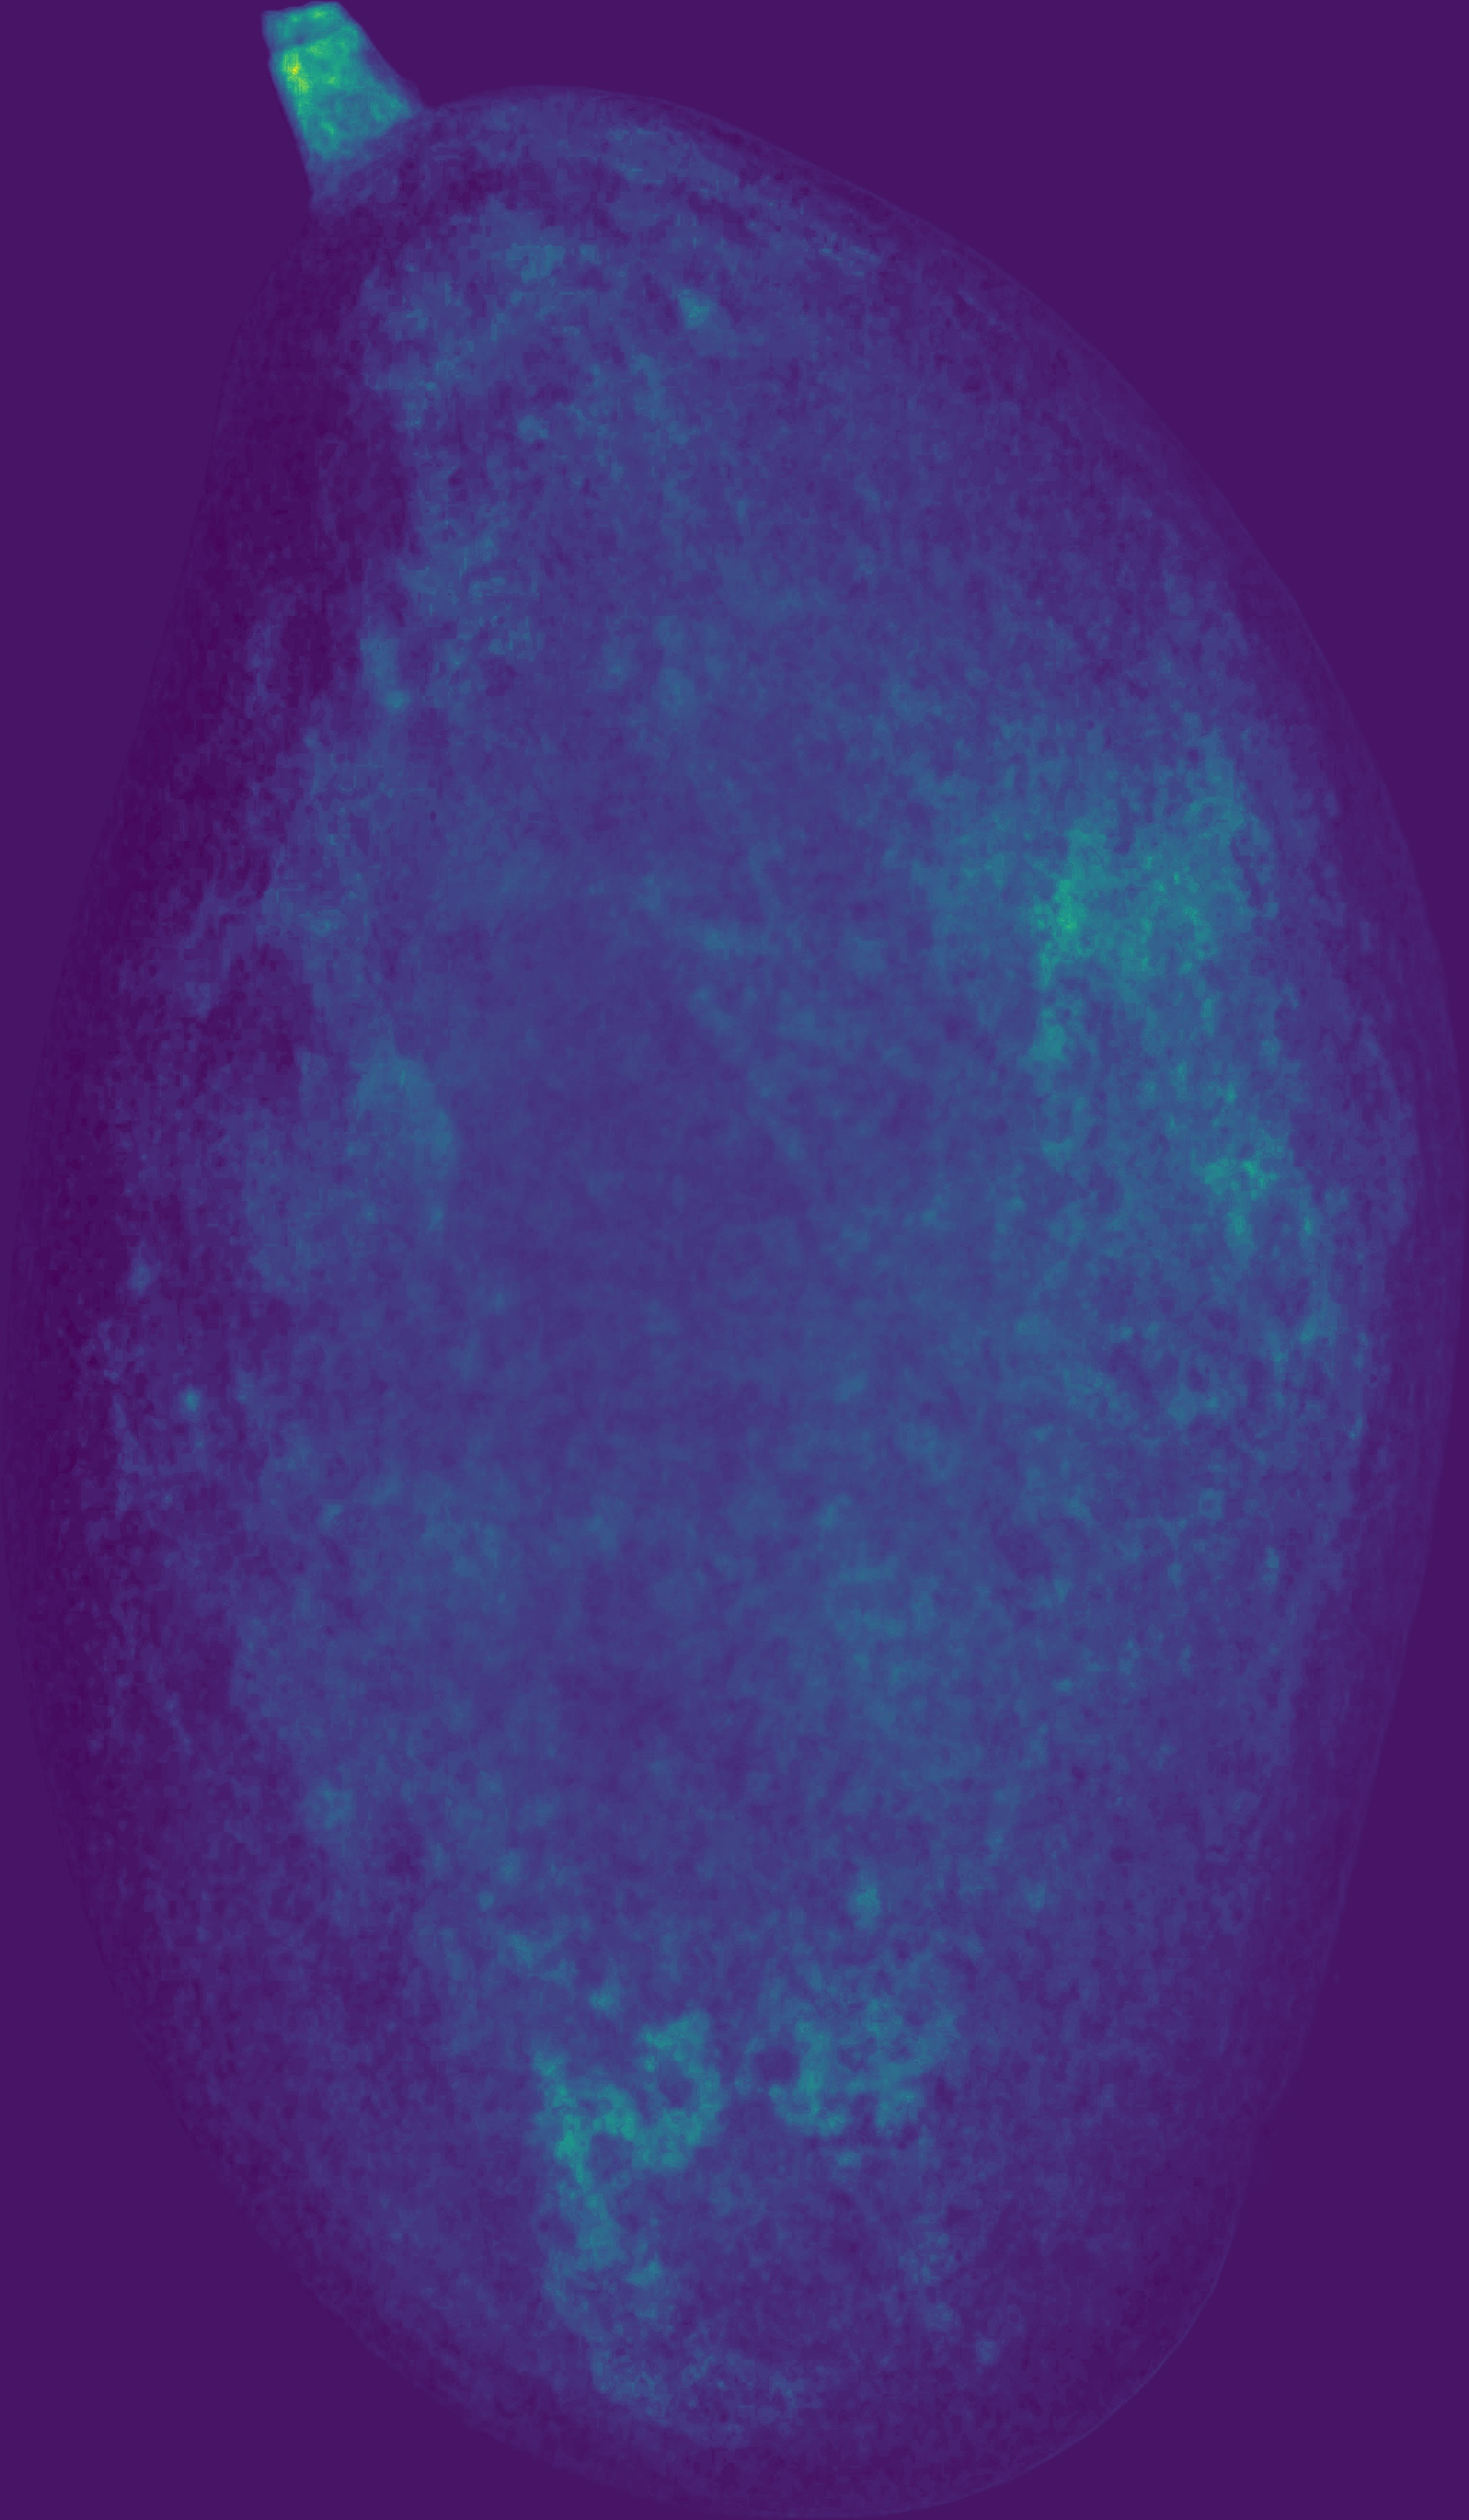
\includegraphics[scale=0.07]{img/RB_rate_img.jpg}
	\legend{\textbf{Fonte:} (Autor, 2019).}\label{fig:rbrate_fig}
\end{figure}

O segundo atributo mais importante, a dimensão de correlação, estima o grau de complexidade de um sistema através da inspeção de pontos distribuídos em um espaço (SRIRAAM, 2012), que neste caso consistem nas intensidades dos pixels. Assim, o quão menos uniforme é a superfície da manga, maior a complexidade. Ademais, os dois outros atributos são associados ao canal azul, em duas regiões específicas a manga. Na Figura \ref{fig:equator_stalk_b}, são especificadas as regiões equatorial e da haste.

\begin{figure}[H]
\centering
	\caption{Regiões equatorial e haste em uma manga representada no canal B.}
	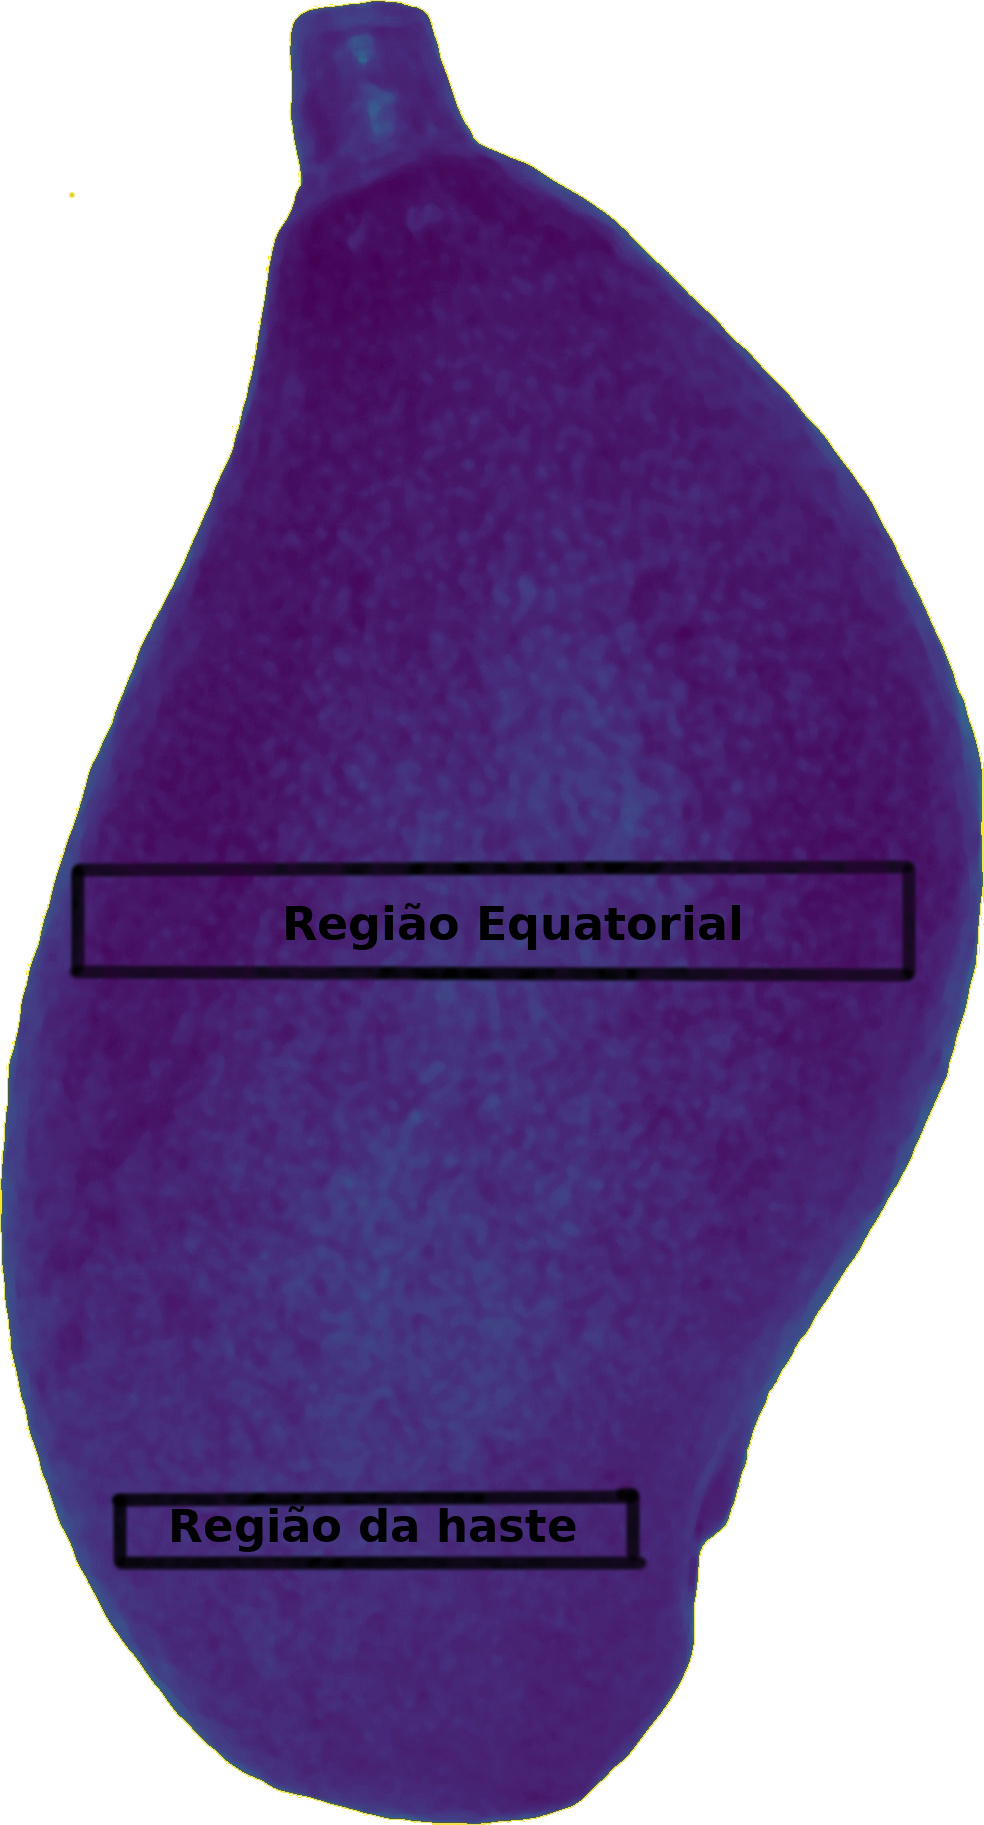
\includegraphics[scale=0.17]{img/B_img.jpg}
	\legend{\textbf{Fonte:} (Autor, 2019).}\label{fig:equator_stalk_b}
\end{figure}

Para entender a relação destas variáveis com o SST, foram plotadas as variações delas de acordo com o atributo de qualidade estudado, conforme mostra a Figura \ref{fig:var_atts}.

\begin{figure}[H]
\centering
	\caption{Variação dos atributos mais importantes para o modelo conforme o SST (a) Taxa R/B (b) Dimensão de correlação (c) Média B na região equatorial (d) Média B na região da haste.}
	\subcaptionbox{}{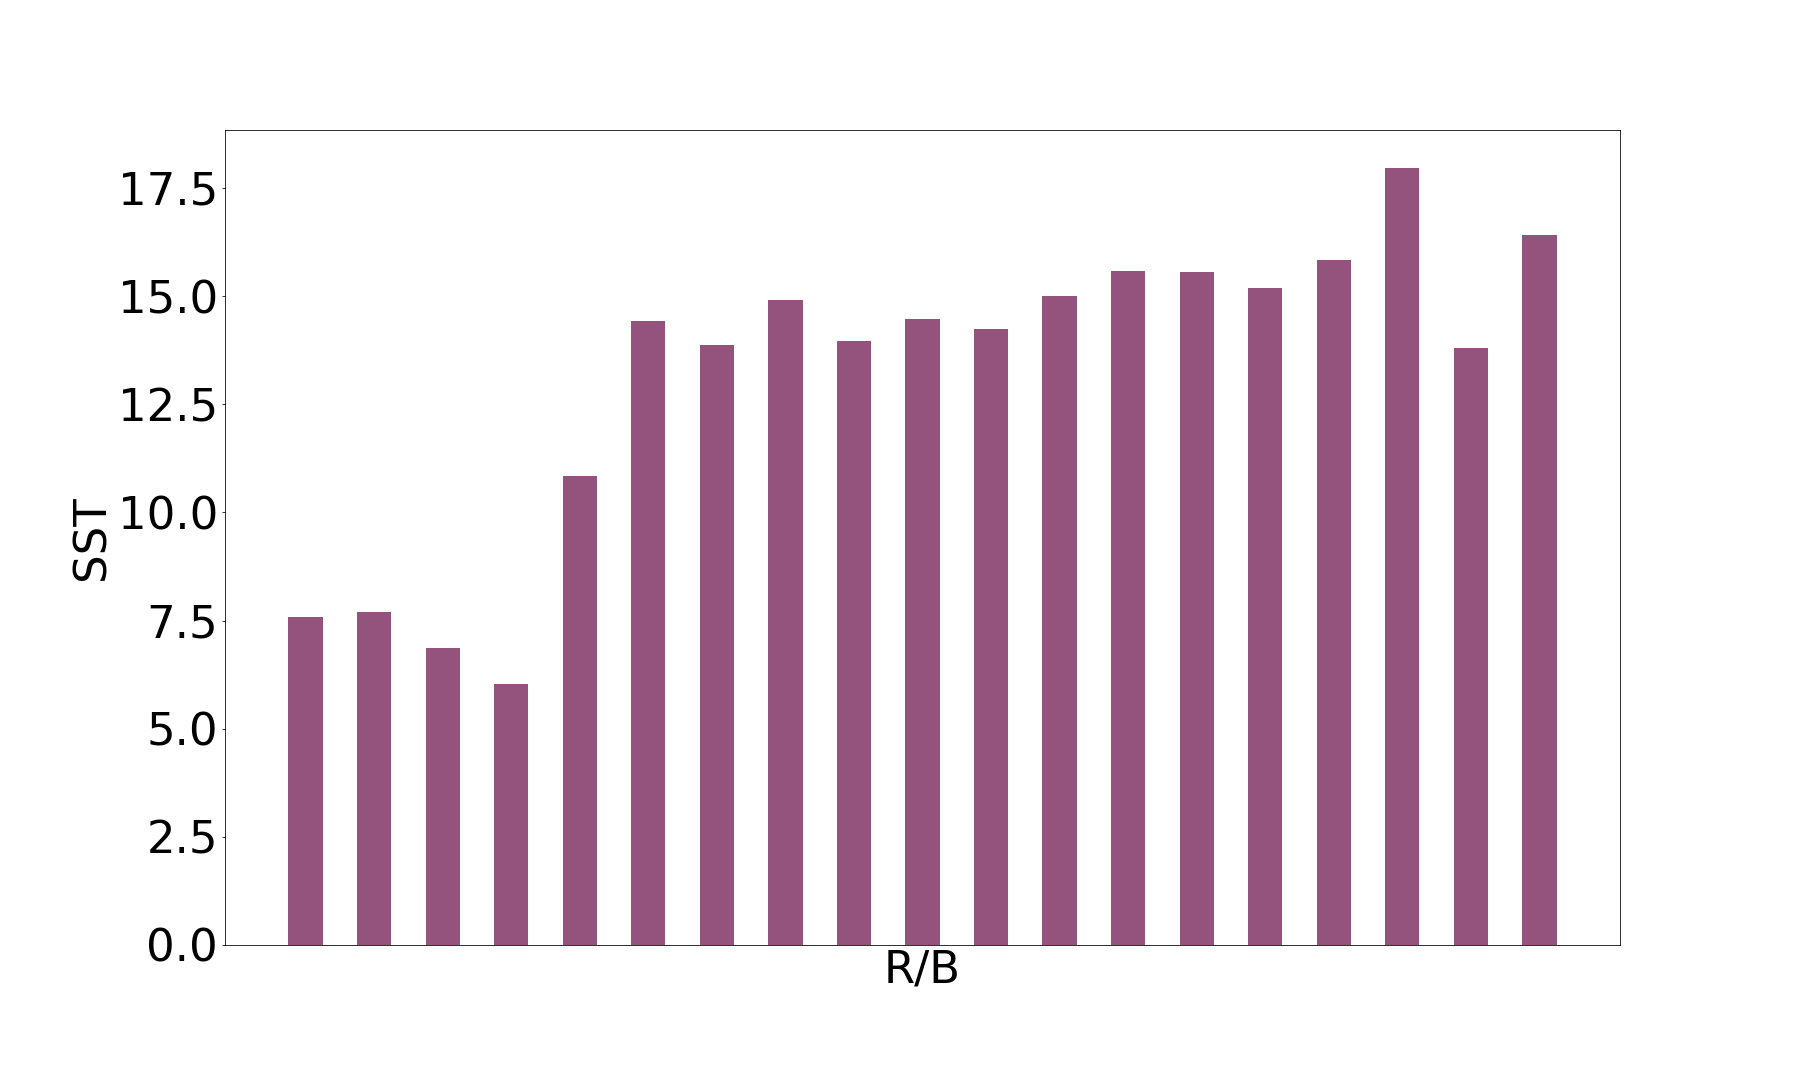
\includegraphics[scale=0.14]{img/RB_sst_palmer.png}}
	\subcaptionbox{}{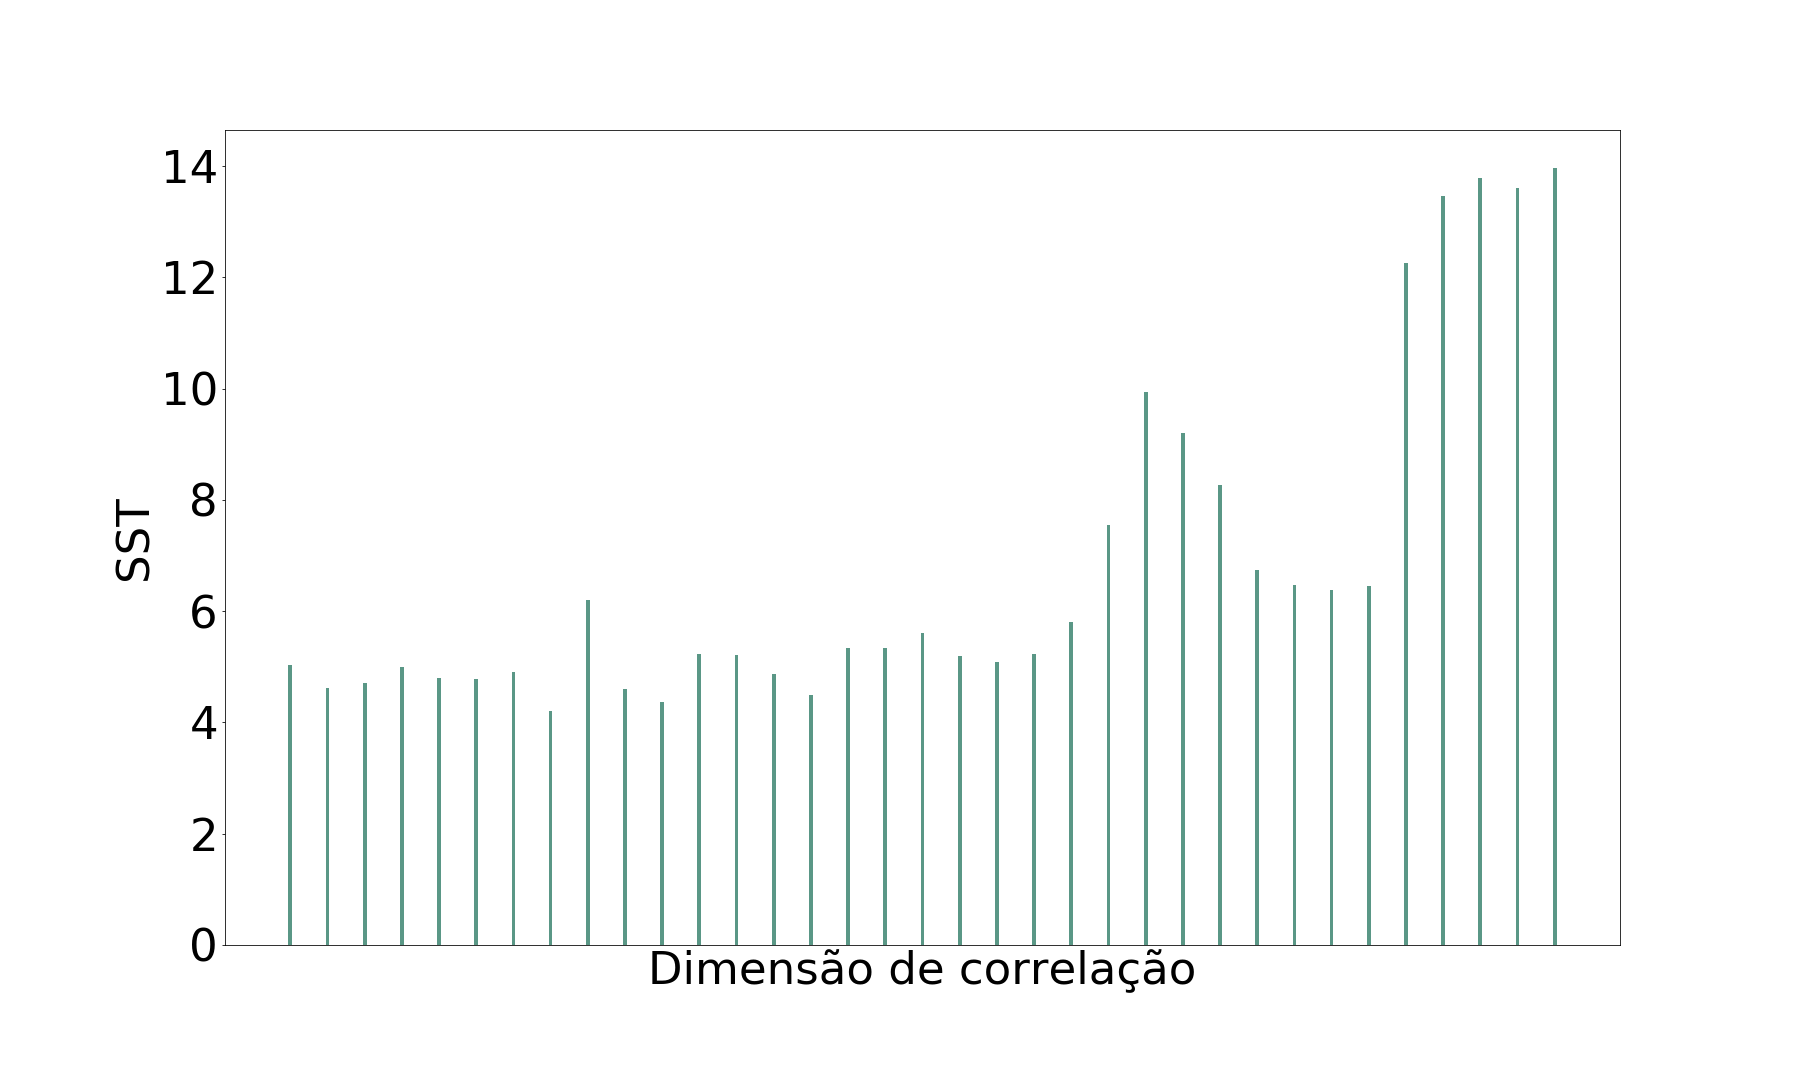
\includegraphics[scale=0.14]{img/cd_sst_palmer.png}}
	\subcaptionbox{}{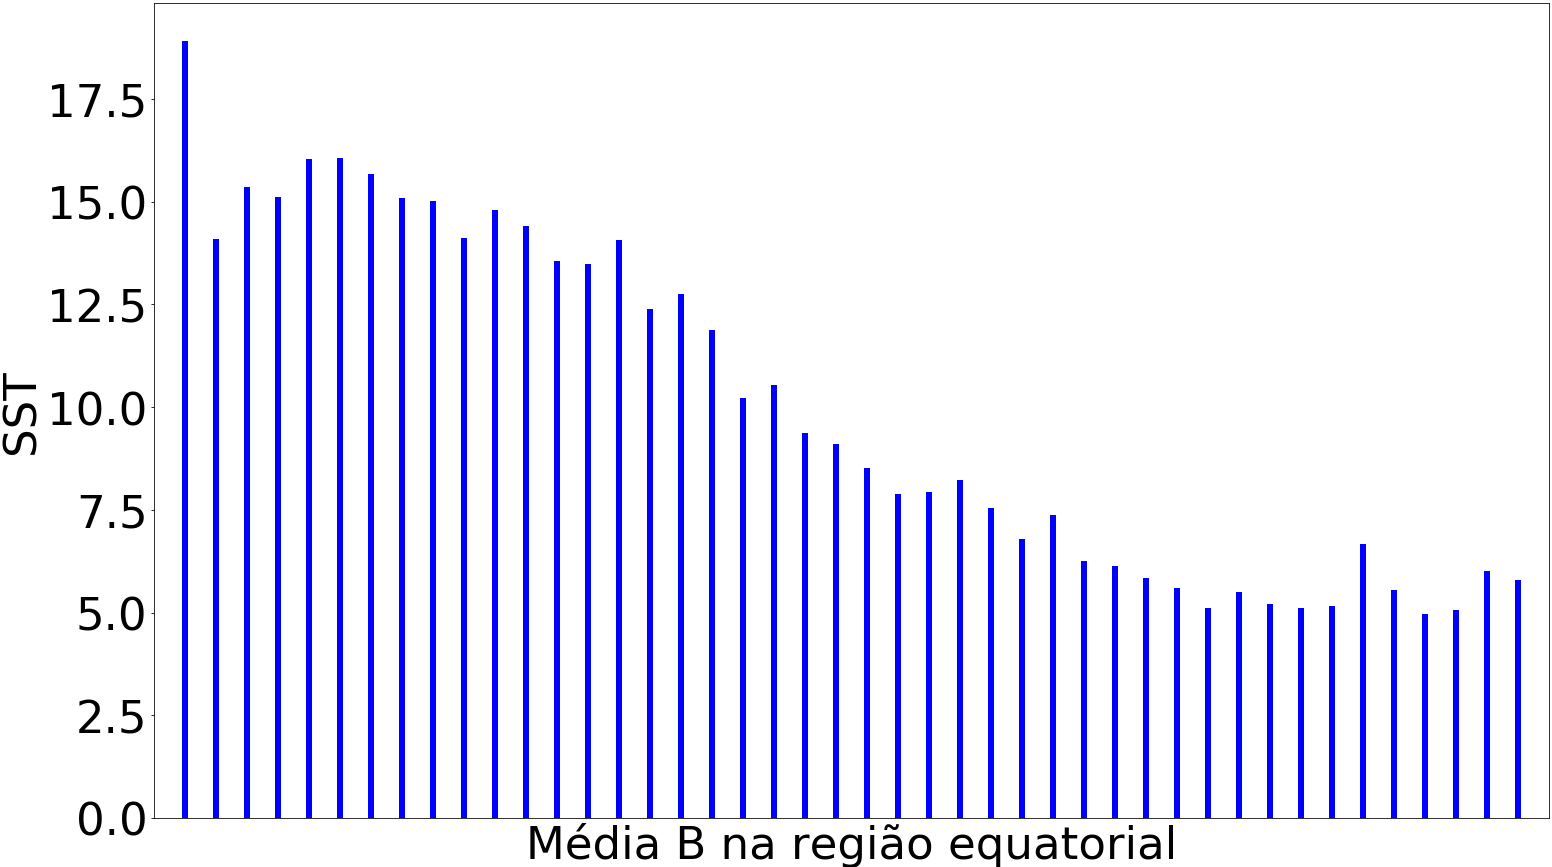
\includegraphics[scale=0.14]{img/equatorb_sst_palmer.png}}
	\subcaptionbox{}{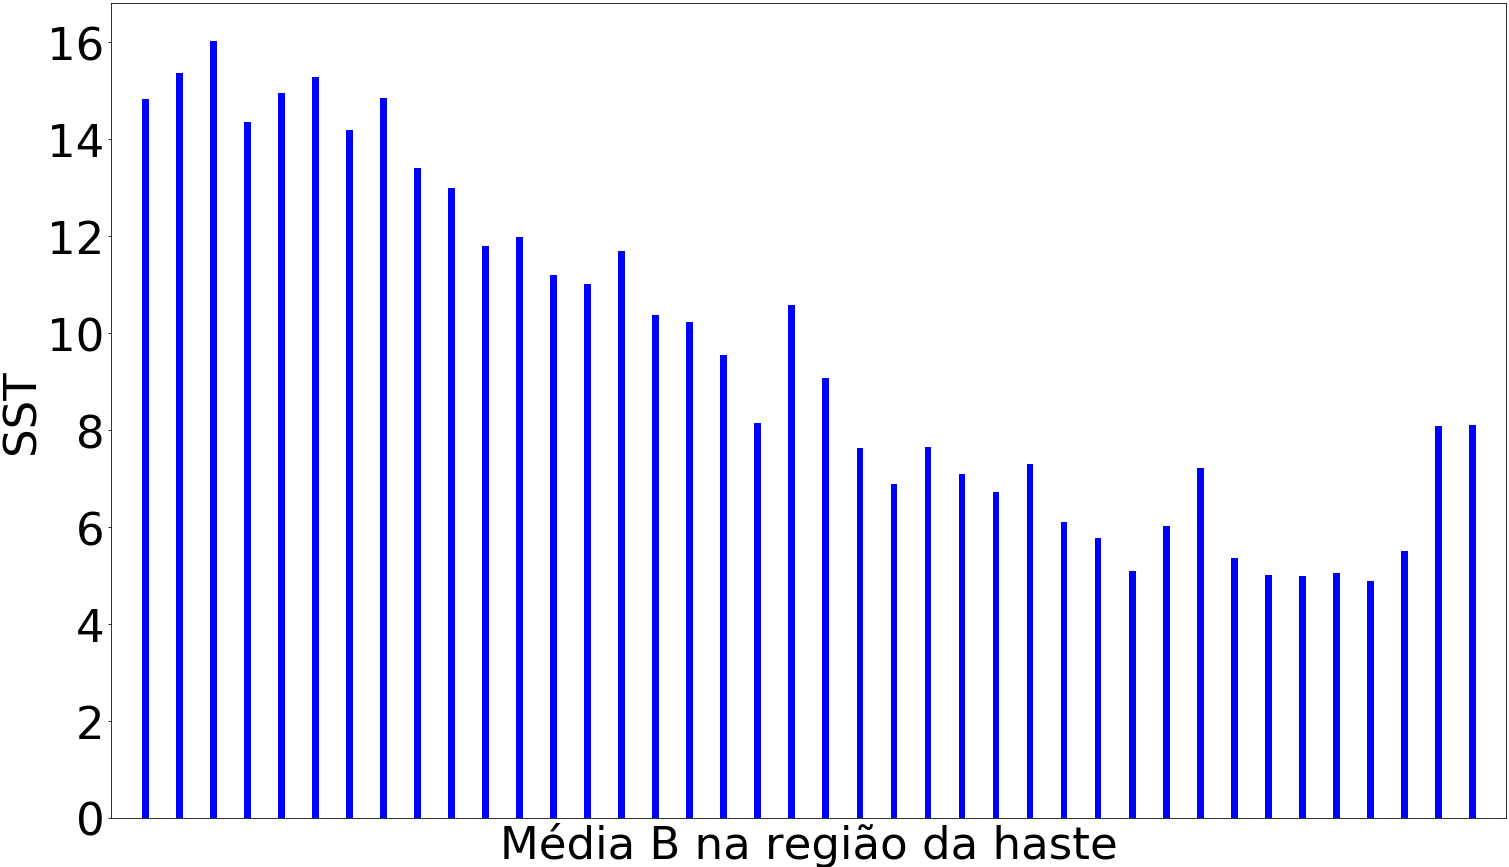
\includegraphics[scale=0.14]{img/stalkb_sst_palmer.png}}
	\legend{\textbf{Fonte:} (Autor, 2019).}\label{fig:var_atts}
\end{figure}

Para a primeira variável, percebe-se que seus valores mais baixos estão associados à mangas verdes, com baixo teor de SST. Com o aumento desse valor, aumenta-se gradativamente o SST, o que corresponde, na imagem, à uma diminuição dos tons amarelados e intensificação dos tons mais roxos. Para a dimensão de correlação, nota-se um comportamento pouco intuitivo e sem padrão, em que os valores de SST permanecem praticamente constantes para vários valores possíveis da variável. Nas outras duas variáveis, há uma diminuição perceptível do nível de SST enquanto a cor azul torna-se menos intensa nas respectivas regiões da manga.

Os demais atributos extraídos apresentaram importâncias menores que 0,01 e foram desconsiderados na construção de um novo modelo de \textit{Random Forest}. O novo modelo apresentou um coeficiente de correlação igual a 0,9752, bastante próximo ao obtido para todas as variáveis.
% \section{Seção de exemplo 1 - Códigos} \label{sec:resex1}

% \subsection{Subseção de exemplo 1 - Inserindo trechos de códigos}
 
% O nosso querido Leonardo Cavalcante providenciou um comando que deixa nossos trechos de códigos bonitinhos e gera um elemento pré-textual de Lista de Códigos. 

% Os códigos são adicionados através do comando seguinte:

% \textbackslash sourcecode\{ Descrição \}\{Label\}\{Linguagem\}\{Arquivo com extensão\}

% Um exemplo pode ser visto no código \ref{cmd:cron} abaixo.

% \sourcecode{Configuração do intervalo de execução no Script Agendador}{cron}{javascript}{cron.js}


% \section{Seção de exemplo 2 - Listas} \label{sec:resex2}

% \subsection{Subseção de exemplo 2 - Lista de itens} 

% Existem alguns tipos de listas no Latex, iremos exemplificar a lista sem numeração (seção \ref{subsubsec:itemize}), a lista enumerada (seção \ref{subsubsec:enumerate}) e a lista mista (seção \ref{subsubsec:mista}). As listas podem ser encadeadas de diversas maneiras,
% de acordo com a necessidade do autor.

% \subsubsection{Subsubseção de exemplo 1 - Lista sem numeração} \label{subsubsec:itemize}

% Este é um exemplo de lista sem numeração.

% \begin{itemize}
% 	\item \textbf{Cadastrar usuário}

% 		\begin{itemize}
%     		\item Atores
% 		    	\begin{itemize}
%     		    	\item Usuário
% 		    	\end{itemize}

% 	    	\item Fluxo de eventos primário
% 			    \begin{itemize}
% 	    		    \item o usuário deve se cadastrar informando seu nome, \textit{e-mail} e senha;
% 		        	\item a API armazena os dados do usuário;
% 		    	    \item o usuário é liberado para realizar o \textit{login}.
% 			    \end{itemize}

%     		\item Fluxo alternativo
% 			    \begin{itemize}
% 		    	   \item o usuário desiste de se cadastrar e cancela o caso de uso clicando no botão voltar.
% 	    		\end{itemize}

% 		\end{itemize}
	
% \end{itemize}

% \subsubsection{Subsubseção de exemplo 2 - Lista enumerada} \label{subsubsec:enumerate}

% Este é um exemplo de lista enumerada.

% \begin{enumerate}
% 	\item O Usuário deseja ver o histórico das variáveis climáticas, então através da interface de usuário escolhe o período ao qual o histórico se refere;
% 	\item A aplicação solicita à API através de uma requisição HTTP contendo o momento de início e o momento do fim do período em seus parâmetros;     			\item A API recebe a solicitação e se comunica com a base de dados, então requere as informações quem possuem a data de leitura no intervalo escolhido;
% 	\item A base de dados retorna os dados em formato Json para a API;
% 	\item A API responde à requisição retornando os dados, também em formato Json, para a aplicação cliente;
% 	\item A aplicação cliente renderiza os gráficos utilizando o conjunto de dados obtidos.
% \end{enumerate}

% \subsubsection{Subsubseção de exemplo 3 - Lista mista} \label{subsubsec:mista}

% Este é um exemplo de lista mista.

% \begin{itemize}
% 	\item \textbf{Cadastrar usuário}

% 		\begin{itemize}
%     		\item Atores
% 		    	\begin{itemize}
%     		    	\item Usuário
% 		    	\end{itemize}

% 	    	\item Fluxo de eventos primário
% 			    \begin{enumerate}
% 	    		    \item o usuário deve se cadastrar informando seu nome, \textit{e-mail} e senha;
% 		        	\item a API armazena os dados do usuário;
% 		    	    \item o usuário é liberado para realizar o \textit{login}.
% 			    \end{enumerate}

%     		\item Fluxo alternativo
% 			    \begin{itemize}
% 		    	   \item o usuário desiste de se cadastrar e cancela o caso de uso clicando no botão voltar.
% 	    		\end{itemize}

% 		\end{itemize}

% 	\item \textbf{Visualizar dados atuais}

% 		\begin{itemize}
% 		    \item Atores
% 	    		\begin{itemize}
% 		    	    \item Usuário
% 			    \end{itemize}
    
% 	    	\item Pré-condições
% 			    \begin{itemize}
% 		     	   \item o usuário deve estar autenticado
% 			    \end{itemize}

% 	    	\item Fluxo de eventos primário
% 			    \begin{enumerate}
% 		    	    \item o usuário deve efetuar o \textit{login} informando o \textit{e-mail} e a senha;
% 	    		    \item caso o usuário não seja autenticado, o sistema informa a respeito de credenciais inválidas e encerra o caso de uso;
% 		    	    \item a API autentica o usuário;
%     			    \item o usuário é liberado para visualizar os dados atuais dos sensores da estação;
% 		        	\item após a visualização o usuário pode finalizar o caso de uso ou efetuar uma nova consulta se desejar.
% 			    \end{enumerate}

%     		\item Fluxo alternativo
% 			    \begin{itemize}
%     			   \item o usuário desiste de visualizar os dados atuais e cancela o caso de uso clicando no botão voltar.
% 			    \end{itemize}

% 		\end{itemize}

% 	\item \textbf{Visualizar histórico}

% 		\begin{itemize}
% 		    \item Atores
% 	    		\begin{itemize}
% 		    	    \item Usuário
% 	    		\end{itemize}

% 	    	\item Pré-condições
%     			\begin{itemize}
% 			        \item o usuário deve estar autenticado
% 			    \end{itemize}

% 		    \item Fluxo de eventos primário
% 			    \begin{enumerate}
% 			        \item o usuário deve efetuar o \textit{login} informando o \textit{e-mail} e a senha;
% 			        \item caso o usuário não seja autenticado, o sistema informa a respeito de credenciais inválidas e encerra o caso de uso;
% 			        \item a API autentica o usuário;
% 			        \item o usuário é liberado para escolher qual período cujo histórico será exibido;
% 			        \item o usuário seleciona as variáveis a serem exibidas no gráficos de linhas;
% 			        \item após a visualização do histórico o usuário pode finalizar o caso de uso se desejar.
% 			    \end{enumerate}

% 		    \item Fluxo alternativo
% 			    \begin{enumerate}
% 			        \item após a escolha do período de exibição do histórico o usuário pode voltar para a tela anterior e escolher um novo período;
% 			        \item o histórico é exibido para o usuário;
% 			        \item após a visualização do histórico o usuário pode finalizar o caso de uso ou efetuar uma nova consulta se desejar.
% 			    \end{enumerate}

% 		    \item Fluxo alternativo
% 			    \begin{enumerate}
% 			        \item o usuário desiste de visualizar o histórico e cancela o caso de uso clicando no botão voltar.
% 			    \end{enumerate}
% 		\end{itemize}
% \end{itemize}